\documentclass[../DefinizioneDiProdotto.tex]{subfiles}
\begin{document}

\section{Schema base di dati}

	Di seguito viene presentata lo schema in UML della base di dati implementata nell'applicativo con SQLite e gestito dal componente \verb|DataManager| e implementata nel server remoto. Lo schema illustra le relazioni tra le entità che costituiscono il grafo rappresentate l'edificio di interesse. Si fa notare che la base di dati non memorizza separatamente gli elementi che compongono i grafi.

	\begin{figure} [h]
			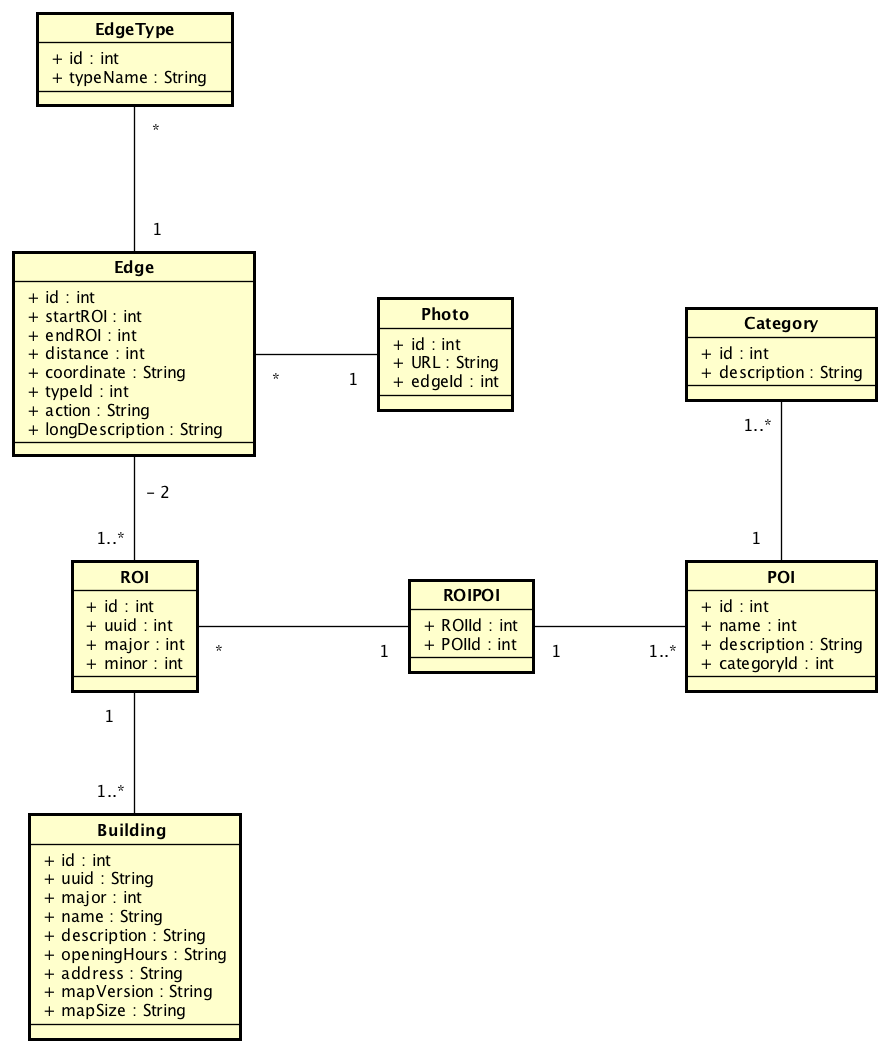
\includegraphics[width=\textwidth]{diagrams/Database}		
			\caption{Schema UML - base di dati}
			\label{Database}
	\end{figure}



\end{document}